\section{CRC cards}
\begin{flushleft}
According to the problem description, each team must construct a CRC card model.For each CRC card, the following must be described: (a) role, (b) responsibilities and the 
rationale for the responsibilities, and (c) collaborations and reasons for collaborating
\end{flushleft}
\begin{flushleft}
    According to the Project documentation of team D, the CRC card model has been constructed. Each of the CRC cards has its role, responsibility and collaborators. But, the rationale behind the responsibility and collaboration is not discussed. 
\end{flushleft}
\begin{figure}[h!]
    \centering
    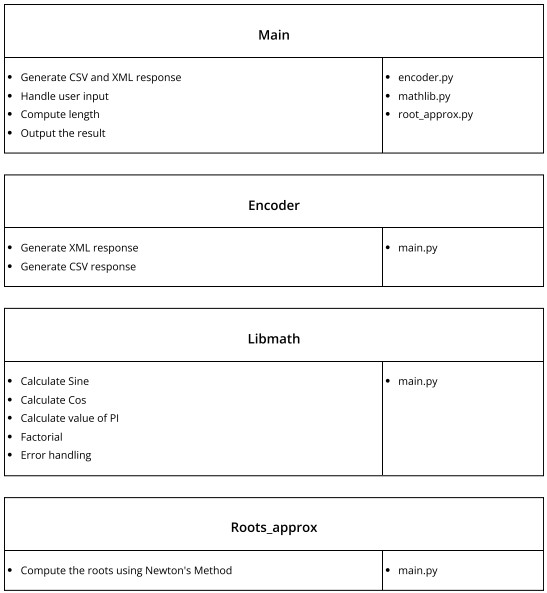
\includegraphics[width=.5\linewidth]{resources/crc_card_team_e.jpg}
    \vspace{.5cm}
    \caption{CRC card model}
    \label{fig:CRC card }
  \end{figure}
  \pagebreak
  \section{Algorithms}
\begin{flushleft}
    Each team must rationalize the selection of each algorithm deployed in source code, and document the 
algorithms using pseudocode. The pseudocode should not be too close to the implementation. 
\end{flushleft}

\begin{flushleft}
    Team D has documented pseudocodes for each of the algorithms they chose. They provided clear and concise justification for each algorithm.
    They also made sure that the algorithm is not close to the implementation.
    For example, in the algorithm for cosine, they provide us with multiple ways of computing cosine including the Taylor series, CORDIC, Lookup table. Out of all these, they chose Taylor series for cosine. They justified it by using the following reason.
    \begin{quote}
        The Taylor series method is considered as one of the most efficient methods for computing cosine,
as it balances accuracy and computational efficiency.It is easy to implement and requires only basic arithmetic
operations, making it a popular choice for software-based implementations of cosine.

    \end{quote}
\end{flushleft}
\section{Source Code}
\subsection{Written from Scratch}
\begin{flushleft}
    Source code S must be written from scratch. S must not make use of any native support in programming languages for trigonometric functions, such as sin(x) and cos(x), and for mathematical constants, such as pi. S must not make use of any application programming interfaces or library functions, other than for input, output, and basic arithmetic.
\end{flushleft}
\begin{flushleft}
    As shown in the below images Source code S is written from the scratch and S did not use any native or external libraries for computing sine, cosine or constant like pi.
\end{flushleft}
\begin{figure}[h!]
    \centering
    \frame{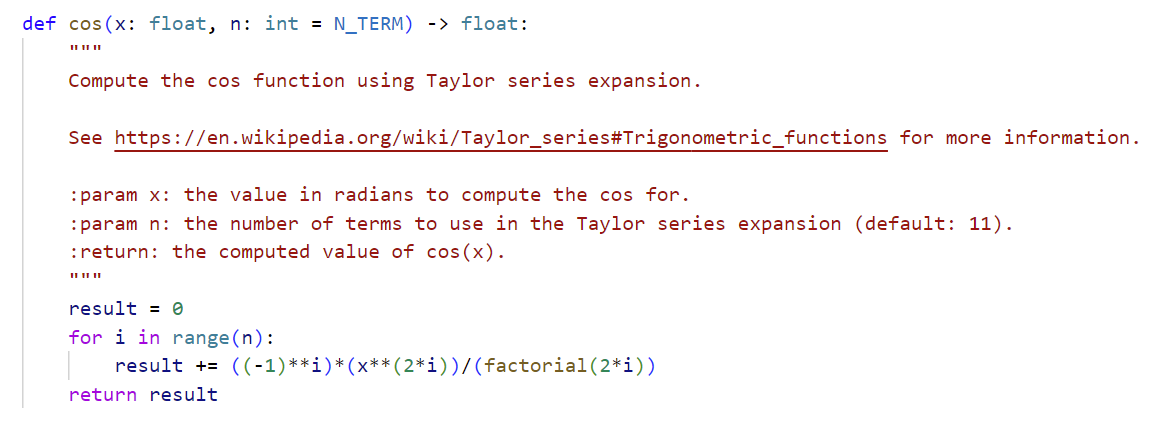
\includegraphics[scale= 0.7]{resources/cos_team_e.png}}
    \vspace{.5cm}
    \caption{Computing value of cos without inbuilt or external libraries}
    \label{fig:cos }
  \end{figure}
  \begin{figure}[h!]
    \centering
    \frame{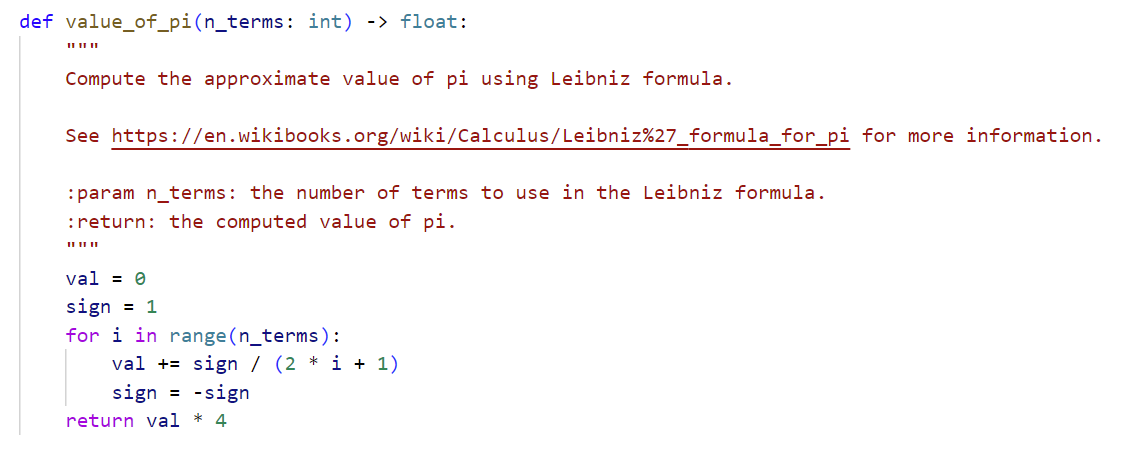
\includegraphics[scale= 0.7]{resources/pi_team_e.png}}
    \vspace{.5cm}
    \caption{Computing value of pi using Taylor series}
    \label{fig:pi }
  \end{figure}
  \subsection{Quality attributes}
  \begin{flushleft}
    Each team has to make sure that the source code is modifiable, readable, reusable, testable, and understandable. They must also ensure that the corresponding program is general, robust, and usable.
  \end{flushleft}
  \begin{flushleft}
    Team D has satisfied the above mentioned conditions.
    \begin{itemize}
         \item \textbf{Modifiability}: By allowing the number of terms in the Taylor series for sine and cosine functions, and the Leibniz formula iteration count for pi to be supplied as arguments, the code becomes more modular and adaptable. This means that the precision of the results can be adjusted easily based on the desired level of accuracy.This flexibility makes the code more versatile and adaptable to different use cases.
    
         \item \textbf{Readability}: The code is legible due to the use of descriptive function names and comments detailing the purpose and rationale of each function. Also, the code complies with PEP 8's style guidelines for Python, making it simple to read and comprehend for other programmers.
    
         \item \textbf{Reusability}: The code's functions for calculating sine, cosine, and pi can be easily reused in future applications by simply importing the file or copying the functions into a new program. The code's modular organization allows individual functions to be reused as needed, as each function serves a specific purpose.
    
         \item \textbf{Testability}: The code is highly testable as each function has a specific purpose and can be evaluated independently. Testing the functions using different input values can help ensure that their outputs are accurate.Overall, the code's modular design and explanatory comments make it straightforward to test and verify the accuracy of its functions.
    
         \item \textbf{Understandability}: The code is designed to be easily understandable by using descriptive function names, comments, and adhering to the PEP 8 style guide. The code's structure and formatting help to clearly explain the rationale behind each function's outcome.
    
        
    \end{itemize}
  \end{flushleft}
  \subsection{Version Control}
  \begin{flushleft}
    Team E has used Git Hub for version control. Git hub is a distributed version control system.
    \begin{figure}[h!]
        \centering
        \frame{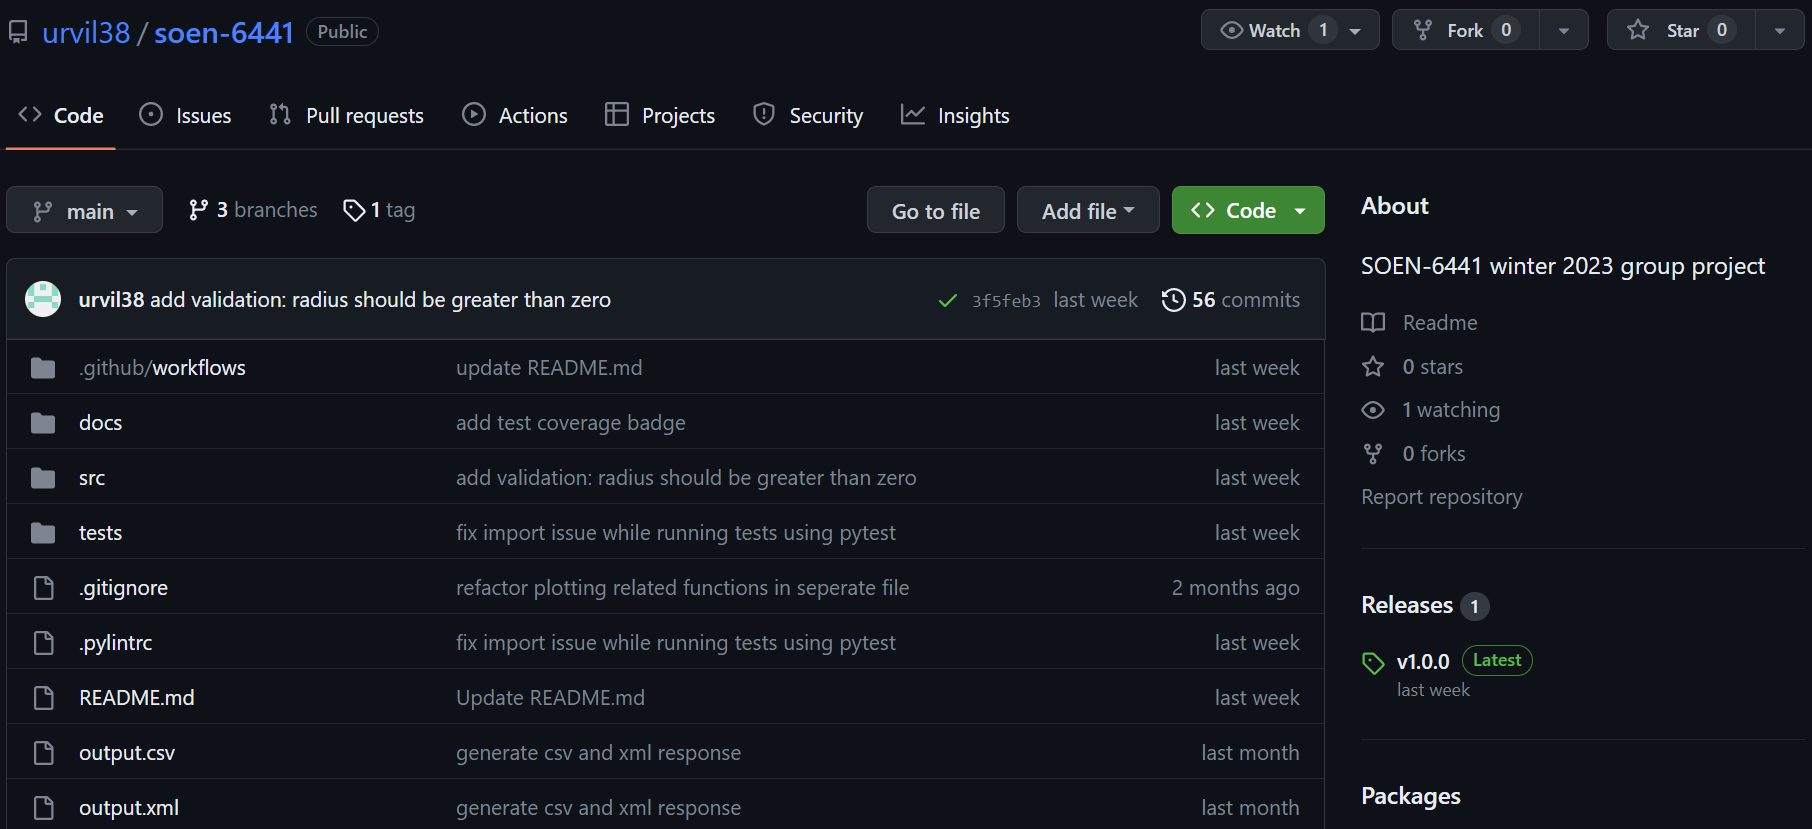
\includegraphics[scale= 0.4]{resources/versioncontrol.png}}
        \caption{Distributed Version Control System}
        \label{fig:GitHub repo}
      \end{figure}
  \end{flushleft}

  \subsection{Programming style}
\begin{flushleft}
    Source Code must follow a style of programming recommended by an authoritative source. (For 
Python, one such authoritative source is PEP 8.) The actual style of programming must 
aim to be consistent across Team.
\end{flushleft}
\begin{flushleft}
    Team D has used PyLint to ensure that they are following PEP 8 guidelines. Running PyLint results in a full score.
    \begin{figure}[h!]
        \centering
        \frame{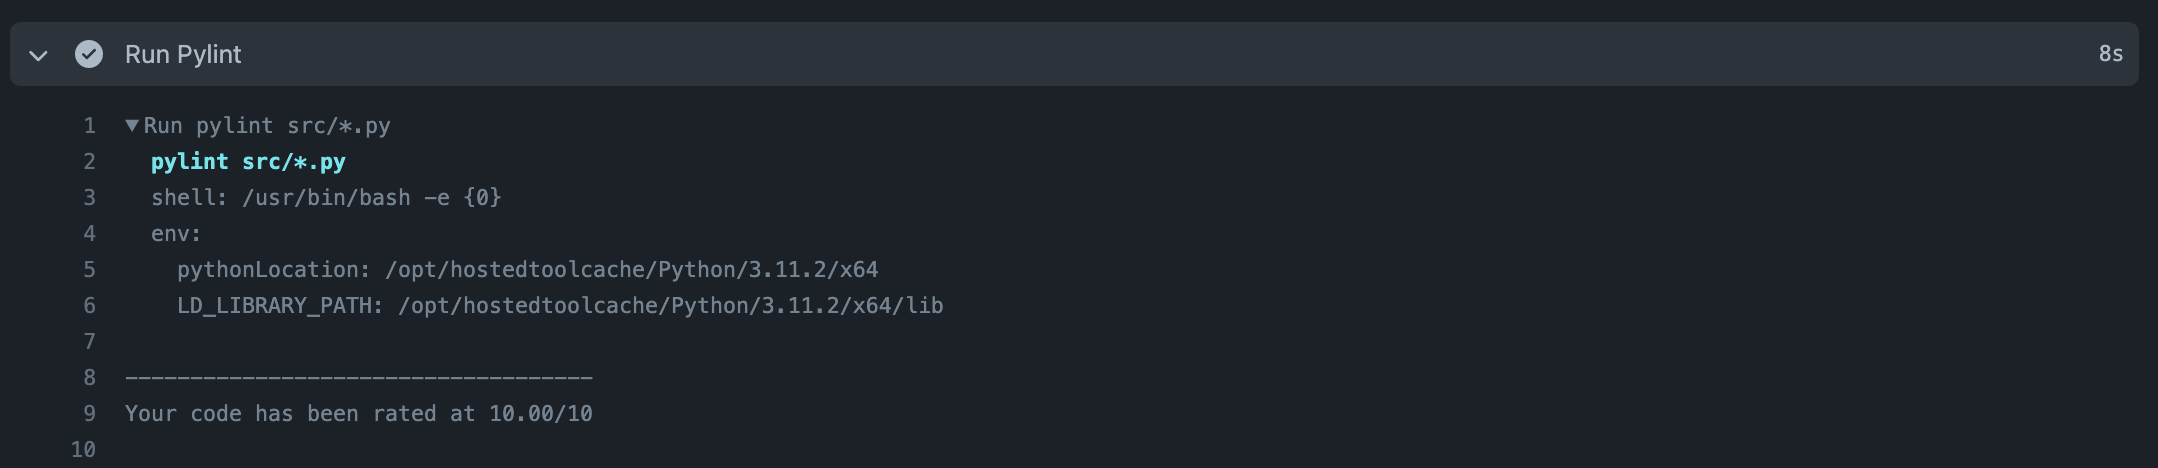
\includegraphics[scale= 0.4]{resources/PEP8.png}}
        \caption{PyLint}
        \label{fig:PyLint}
      \end{figure}
\end{flushleft}
\subsection{Documentation}
\begin{flushleft}
    Each team must be documented appropriately using a standard documentation system. Here team D has used PyDocs to document their source code.
    \begin{figure}[h!]
        \centering
        \frame{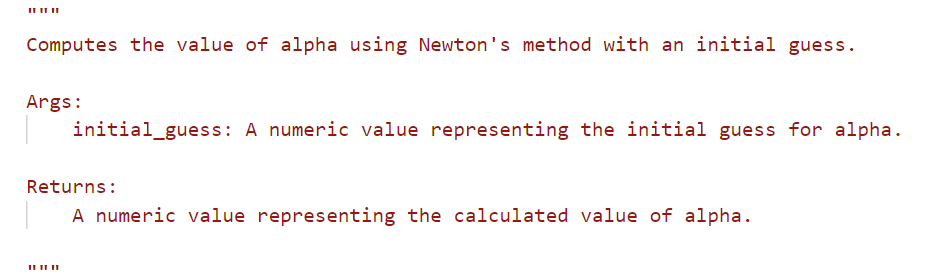
\includegraphics[scale= 0.7]{resources/docstrings.png}}
        \vspace{.5cm}
        \caption{Doc Strings}
        \label{fig:docstrings }
    \end{figure}
\end{flushleft}
\subsection{Error Handling}
\begin{flushleft}
    Team D has properly handled exceptions and errors. They also provide intuitive messages to the end users.
    \begin{figure}[h!]
        \centering
        \frame{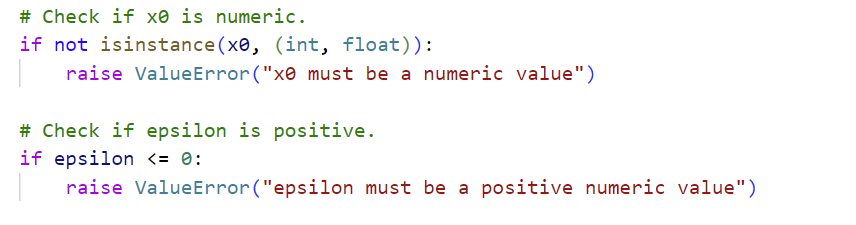
\includegraphics[scale= 0.7]{resources/errorhandeling.png}}
        \vspace{.5cm}
        \caption{Error handling}
        \label{fig:errpr handelling }
    \end{figure}
\end{flushleft}
\subsection{Processing source code}
\begin{flushleft}
    The GitHub repository of team D has clear and concise instructions for processing source code.
    \begin{figure}[h!]
        \centering
        \frame{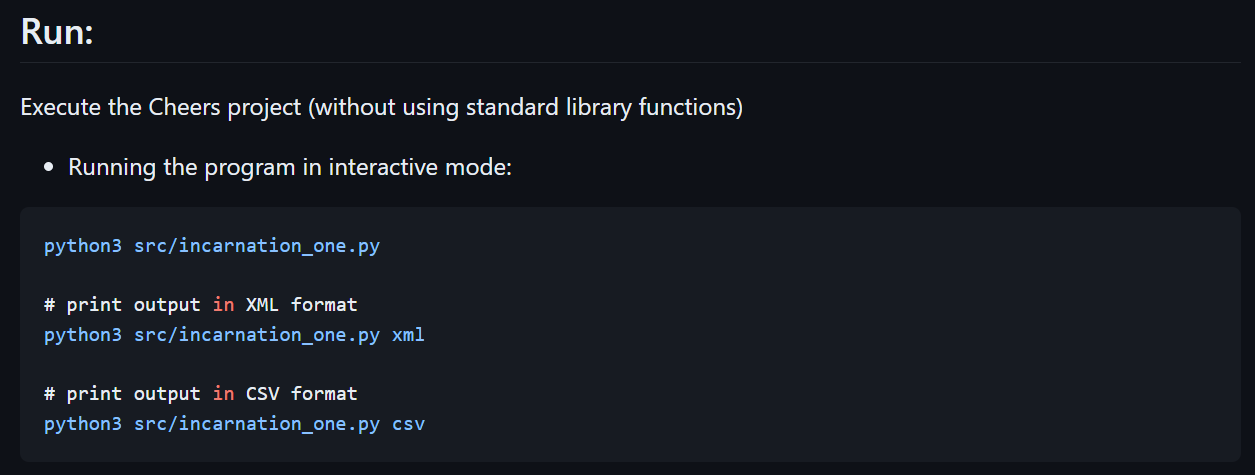
\includegraphics[scale= 0.7]{resources/runinstructions.png}}
        \vspace{.5cm}
        \caption{Instructions for executing source code}
        \label{fig:run instructions }
    \end{figure}
\end{flushleft}
\subsection{IDE independent}
\begin{flushleft}
    All the dependencies used for the source code are mentioned in the requirements.txt file. All the required dependencies are independent of the development environment.
\end{flushleft}
  \section{Output}
  \subsection{incarnation 1}
  \begin{flushleft}
    Each team must provide a sample output for different values of R. The output must be in structured plain text. Team E has provided a sample output for various values of radius.
  \end{flushleft}
  \begin{figure}[h!]
    \centering
    \frame{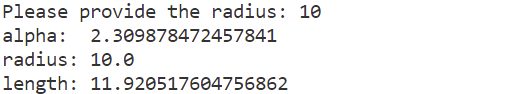
\includegraphics[scale= 0.7]{resources/sample output.png}}
    \vspace{.5cm}
    \caption{Sample output}
    \label{fig:cos }
  \end{figure}
  \subsection{Incarnation 2}
  \begin{flushleft}
    T must provide a sample output, say, for different values of R. The output of P must be expressed in XML. This output must be valid with respect to some XML DTD.
  \end{flushleft}
  \begin{flushleft}
    Team E has generated the output for incarnation 2 in form of an XML document. The output is validated using an XML DTD
  \end{flushleft}
  \begin{figure}[h!]
    \centering
    \frame{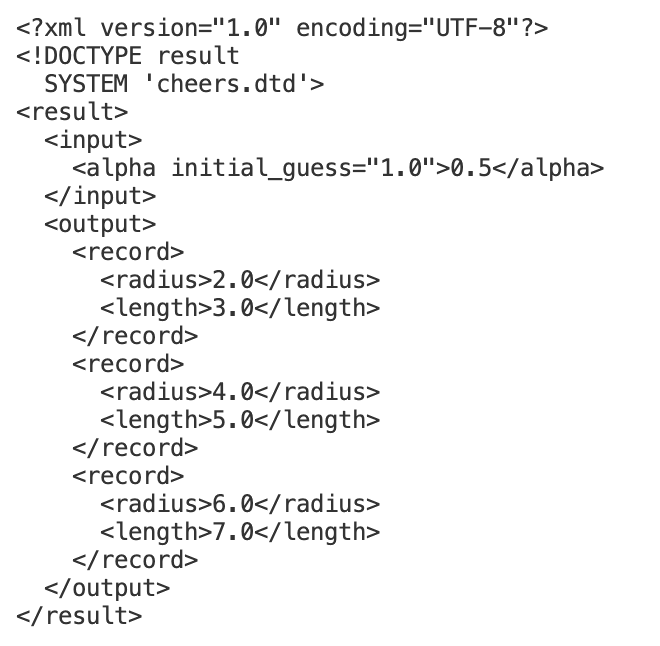
\includegraphics[scale= 0.4]{resources/expected/expected_xml.png}}
    \caption{Expected XML}
    \label{fig:XML output}
  \end{figure}
  \begin{figure}[h!]
    \centering
    \frame{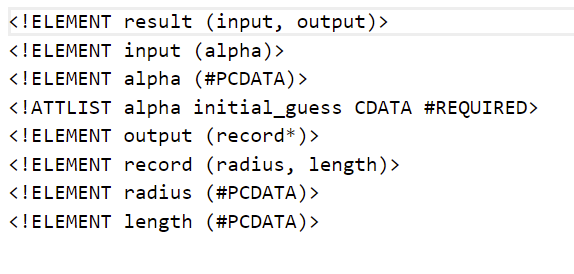
\includegraphics[scale= 0.4]{resources/xml_dtd.png}}
    \caption{XML DTD}
    \label{fig:XML DTD}
  \end{figure}
 